% Options for packages loaded elsewhere
\PassOptionsToPackage{unicode}{hyperref}
\PassOptionsToPackage{hyphens}{url}
%
\documentclass[
]{article}
\usepackage{amsmath,amssymb}
\usepackage{iftex}
\ifPDFTeX
  \usepackage[T1]{fontenc}
  \usepackage[utf8]{inputenc}
  \usepackage{textcomp} % provide euro and other symbols
\else % if luatex or xetex
  \usepackage{unicode-math} % this also loads fontspec
  \defaultfontfeatures{Scale=MatchLowercase}
  \defaultfontfeatures[\rmfamily]{Ligatures=TeX,Scale=1}
\fi
\usepackage{lmodern}
\ifPDFTeX\else
  % xetex/luatex font selection
\fi
% Use upquote if available, for straight quotes in verbatim environments
\IfFileExists{upquote.sty}{\usepackage{upquote}}{}
\IfFileExists{microtype.sty}{% use microtype if available
  \usepackage[]{microtype}
  \UseMicrotypeSet[protrusion]{basicmath} % disable protrusion for tt fonts
}{}
\makeatletter
\@ifundefined{KOMAClassName}{% if non-KOMA class
  \IfFileExists{parskip.sty}{%
    \usepackage{parskip}
  }{% else
    \setlength{\parindent}{0pt}
    \setlength{\parskip}{6pt plus 2pt minus 1pt}}
}{% if KOMA class
  \KOMAoptions{parskip=half}}
\makeatother
\usepackage{xcolor}
\usepackage[margin=1in]{geometry}
\usepackage{color}
\usepackage{fancyvrb}
\newcommand{\VerbBar}{|}
\newcommand{\VERB}{\Verb[commandchars=\\\{\}]}
\DefineVerbatimEnvironment{Highlighting}{Verbatim}{commandchars=\\\{\}}
% Add ',fontsize=\small' for more characters per line
\usepackage{framed}
\definecolor{shadecolor}{RGB}{248,248,248}
\newenvironment{Shaded}{\begin{snugshade}}{\end{snugshade}}
\newcommand{\AlertTok}[1]{\textcolor[rgb]{0.94,0.16,0.16}{#1}}
\newcommand{\AnnotationTok}[1]{\textcolor[rgb]{0.56,0.35,0.01}{\textbf{\textit{#1}}}}
\newcommand{\AttributeTok}[1]{\textcolor[rgb]{0.13,0.29,0.53}{#1}}
\newcommand{\BaseNTok}[1]{\textcolor[rgb]{0.00,0.00,0.81}{#1}}
\newcommand{\BuiltInTok}[1]{#1}
\newcommand{\CharTok}[1]{\textcolor[rgb]{0.31,0.60,0.02}{#1}}
\newcommand{\CommentTok}[1]{\textcolor[rgb]{0.56,0.35,0.01}{\textit{#1}}}
\newcommand{\CommentVarTok}[1]{\textcolor[rgb]{0.56,0.35,0.01}{\textbf{\textit{#1}}}}
\newcommand{\ConstantTok}[1]{\textcolor[rgb]{0.56,0.35,0.01}{#1}}
\newcommand{\ControlFlowTok}[1]{\textcolor[rgb]{0.13,0.29,0.53}{\textbf{#1}}}
\newcommand{\DataTypeTok}[1]{\textcolor[rgb]{0.13,0.29,0.53}{#1}}
\newcommand{\DecValTok}[1]{\textcolor[rgb]{0.00,0.00,0.81}{#1}}
\newcommand{\DocumentationTok}[1]{\textcolor[rgb]{0.56,0.35,0.01}{\textbf{\textit{#1}}}}
\newcommand{\ErrorTok}[1]{\textcolor[rgb]{0.64,0.00,0.00}{\textbf{#1}}}
\newcommand{\ExtensionTok}[1]{#1}
\newcommand{\FloatTok}[1]{\textcolor[rgb]{0.00,0.00,0.81}{#1}}
\newcommand{\FunctionTok}[1]{\textcolor[rgb]{0.13,0.29,0.53}{\textbf{#1}}}
\newcommand{\ImportTok}[1]{#1}
\newcommand{\InformationTok}[1]{\textcolor[rgb]{0.56,0.35,0.01}{\textbf{\textit{#1}}}}
\newcommand{\KeywordTok}[1]{\textcolor[rgb]{0.13,0.29,0.53}{\textbf{#1}}}
\newcommand{\NormalTok}[1]{#1}
\newcommand{\OperatorTok}[1]{\textcolor[rgb]{0.81,0.36,0.00}{\textbf{#1}}}
\newcommand{\OtherTok}[1]{\textcolor[rgb]{0.56,0.35,0.01}{#1}}
\newcommand{\PreprocessorTok}[1]{\textcolor[rgb]{0.56,0.35,0.01}{\textit{#1}}}
\newcommand{\RegionMarkerTok}[1]{#1}
\newcommand{\SpecialCharTok}[1]{\textcolor[rgb]{0.81,0.36,0.00}{\textbf{#1}}}
\newcommand{\SpecialStringTok}[1]{\textcolor[rgb]{0.31,0.60,0.02}{#1}}
\newcommand{\StringTok}[1]{\textcolor[rgb]{0.31,0.60,0.02}{#1}}
\newcommand{\VariableTok}[1]{\textcolor[rgb]{0.00,0.00,0.00}{#1}}
\newcommand{\VerbatimStringTok}[1]{\textcolor[rgb]{0.31,0.60,0.02}{#1}}
\newcommand{\WarningTok}[1]{\textcolor[rgb]{0.56,0.35,0.01}{\textbf{\textit{#1}}}}
\usepackage{graphicx}
\makeatletter
\newsavebox\pandoc@box
\newcommand*\pandocbounded[1]{% scales image to fit in text height/width
  \sbox\pandoc@box{#1}%
  \Gscale@div\@tempa{\textheight}{\dimexpr\ht\pandoc@box+\dp\pandoc@box\relax}%
  \Gscale@div\@tempb{\linewidth}{\wd\pandoc@box}%
  \ifdim\@tempb\p@<\@tempa\p@\let\@tempa\@tempb\fi% select the smaller of both
  \ifdim\@tempa\p@<\p@\scalebox{\@tempa}{\usebox\pandoc@box}%
  \else\usebox{\pandoc@box}%
  \fi%
}
% Set default figure placement to htbp
\def\fps@figure{htbp}
\makeatother
\setlength{\emergencystretch}{3em} % prevent overfull lines
\providecommand{\tightlist}{%
  \setlength{\itemsep}{0pt}\setlength{\parskip}{0pt}}
\setcounter{secnumdepth}{-\maxdimen} % remove section numbering
\usepackage{bookmark}
\IfFileExists{xurl.sty}{\usepackage{xurl}}{} % add URL line breaks if available
\urlstyle{same}
\hypersetup{
  pdftitle={Priced Out: Housing Affordability in the Netherlands},
  hidelinks,
  pdfcreator={LaTeX via pandoc}}

\title{Priced Out: Housing Affordability in the Netherlands}
\usepackage{etoolbox}
\makeatletter
\providecommand{\subtitle}[1]{% add subtitle to \maketitle
  \apptocmd{\@title}{\par {\large #1 \par}}{}{}
}
\makeatother
\subtitle{Tutorial group: Tutorial 1 Group 6\\
Tutorial lecturer: Jack Fitzgerald}
\author{Daan Blok (2821386), Daniel ten Broeke (2823206), Dries A. M.
Berns (2769645),\\
Konstantinos Ntovas (2860092), Mariah P. Mendoza (2856166), Sofie A.
Hopman (2745673),\\
Vlad A. Partenie (2838992)}
\date{2025-06-24}

\begin{document}
\maketitle

\section{Part 1 - Identifying a Social
Problem}\label{part-1---identifying-a-social-problem}

The housing market in the Netherlands is currently facing significant
problems, especially for young people. There are long waiting lists for
rental housing, and in addition, there are high rental prices in the
private sector. The prices of owner-occupied homes have risen sharply in
recent years, making it increasingly difficult for young people and
young adults to find affordable housing (Wat Zijn Gevolgen van de
Onzekere Woningmarkt Voor Jongeren? \textbar{} Nederlands
Jeugdinstituut, n.d.-b). This has led to a historic low in the number of
young people who have purchased a home. According to the CBS, there is a
shortage of approximately 315,000 homes in the Netherlands (Wat Zijn
Gevolgen van de Onzekere Woningmarkt Voor Jongeren? \textbar{}
Nederlands Jeugdinstituut, n.d.-b). Furthermore the research by Wiesel
et al.~(2021) highlights that there are significant differences between
generations regarding income inequality. Baby boomers have benefited
from relatively affordable housing, while younger generations, such as
Generation X and millennials, face greater challenges in covering
housing costs. This has direct implications for their economic
opportunities. The rising house prices and increasing housing costs have
contributed to the growing inequality in the housing market. Households
with middle incomes are also experiencing increasing problems. Many of
these households fall between the cracks, as their income is too high
for social rental housing but too low for the private rental market.
This results in limited access to affordable housing (Schilder et al.,
n.d.). Although the social rental sector in the Netherlands offers
affordable rents in absolute terms, the pressure on this sector is
increasing, particularly due to the growing number of households that
rely on social housing (Schilder et al., n.d.). The combination of these
factors makes the situation in the housing market particularly urgent
and calls for attention from policymakers to address the issues and
ensure access to affordable housing for young people and other
vulnerable groups.

\section{Part 2 - Data Sourcing}\label{part-2---data-sourcing}

\subsection{2.1 Load in the data}\label{load-in-the-data}

\begin{Shaded}
\begin{Highlighting}[]
\NormalTok{load\_cbs\_raw }\OtherTok{\textless{}{-}} \ControlFlowTok{function}\NormalTok{(table\_id) \{}
  \FunctionTok{cbs\_get\_data}\NormalTok{(table\_id, }\AttributeTok{typed =} \ConstantTok{FALSE}\NormalTok{)}
\NormalTok{\}}

\NormalTok{raw\_tables }\OtherTok{\textless{}{-}} \FunctionTok{suppressWarnings}\NormalTok{(}\FunctionTok{map}\NormalTok{(table\_ids, load\_cbs\_raw))}
\CommentTok{\#loads the datasets through their predefined ids}
\end{Highlighting}
\end{Shaded}

\subsection{2.2 \& 2.3 Short summary of the dataset and the variables
included
described}\label{short-summary-of-the-dataset-and-the-variables-included-described}

Three external datasets are retrieved directly from CBS via the
internet, using a predefined vector of dataset codes to automate access
and ensure reproducibility. The specific codes used are listed in the
corresponding vector \texttt{table\_ids}. These datasets are compiled by
CBS using a combination of integral administrative sources and, in some
cases, survey data. For example, the Integrale inkomens- en
vermogensstatistiek (Pouwels-Urlings, 2021) is based on comprehensive
records from institutions such as the Belastingdienst (Dutch Tax
Authority), Dienst Uitvoering Onderwijs (DUO), Uitvoeringsinstituut
Werknemersverzekeringen (UWV), and the Basisregistratie Personen (BRP).
The Huizenprijsindex bestaande koopwoningen (83625NED) relies on
transaction data from the Kadaster (Centraal Bureau voor de Statistiek,
2008), which is updated monthly and considered immediately final.
Meanwhile, the Stelsel van Sociaal-statistische Bestanden (Bakker et
al., 2014) draws primarily on administrative registrations, but also
incorporates data from the Enquête Beroepsbevolking (EBB -- Labour Force
Survey). These sources ensure the statistical accuracy and reliability
of the datasets used in this analysis.

The first dataset contains three variables: \texttt{RegioS}, which
denotes region codes defined in the dataset's metadata and linked to the
\texttt{province\_map}; \texttt{Perioden}, which covers yearly data from
1995 to 2024, using the CBS format (e.g., 1995JJ00) that corresponds to
calendar years; and \texttt{GemiddeldeVerkoopprijs\_1}, which provides
average sale prices of homes per region and year.

The second dataset is more detailed, with 20 variables related to
household characteristics. It includes \texttt{RegioS} and
\texttt{Perioden} beginning from 2011, and
\texttt{KenmerkenVanHuishoudens}, a coded variable that identifies
household types---filtered for relevant categories using
\texttt{kenmerken\_map}. The variable \texttt{Populatie} distinguishes
subpopulations, such as private households with or without students.
Additionally, it contains both absolute
(\texttt{ParticuliereHuishoudens\_1}) and relative
(\texttt{ParticuliereHuishoudensRelatief\_2}) household counts.
Crucially, this dataset includes several income indicators, such as
average and median standardised income
(\texttt{GemiddeldGestandaardiseerdInkomen\_3},
\texttt{MediaanGestandaardiseerdInkomen\_4}) and income decile groups
(\texttt{GestandaardiseerdInkomen1e10Groep\_7} to \texttt{\_16}), making
it an essential resource for assessing income distribution in relation
to housing affordability.

The third dataset complements the other two by focusing on the
demographic composition of households and living arrangements. It
includes 16 variables and covers the period from 2000 onward. The
variable \texttt{Geslacht} distinguishes between all persons, men, and
women using CBS codes (e.g., T001038, 3000, 4000). Age groups are
captured via \texttt{Leeftijd}, defined in the metadata and referenced
with the \texttt{age\_map} vector. Like the others, it includes
\texttt{RegioS} and \texttt{Perioden}. It offers a breakdown of
household roles and living arrangements, including single-person
households (\texttt{Alleenstaand\_4}), cohabiting individuals, children
living at home, and various couple structures (e.g., married/unmarried,
with/without children). It also includes more specific roles such as
single parents (\texttt{OuderInEenouderhuishouden\_10}) and individuals
in institutional households. This dataset enables detailed insight into
who lives on themselves, how household compositions shift over time, and
how these patterns differ by age and gender---important factors when
evaluating housing needs and affordability.

Together, these three datasets are highly complementary. The first
provides a direct measure of housing prices, the second supplies
critical socioeconomic and income-related variables, and the third
offers insight into demographic and household structure changes over
time. Their shared use of \texttt{RegioS} and \texttt{Perioden} allows
for integration across geographic and temporal dimensions, making them
well-suited for a multidimensional analysis of housing affordability.

However, several limitations must be acknowledged. First, the time
coverage is inconsistent: the first dataset spans 1995--2024, the second
starts in 2011, and the third from 2000. This mismatch complicates
long-term trend analysis, especially for integrated models. Second, not
all time points have complete data---some values are missing or not
filled in. Third, the datasets contain many variables that are
irrelevant to the specific research focus and must be filtered out,
increasing preprocessing time. Lastly, while administrative sources
offer consistency, they may overlook informal living situations or
alternative housing arrangements not captured in official registers.
Despite these challenges, the richness, credibility, and compatibility
of these datasets make them an excellent foundation for a thorough,
data-driven analysis of housing affordability in the Netherlands.

\section{Part 3 - Quantifying}\label{part-3---quantifying}

\subsection{3.1 Data cleaning}\label{data-cleaning}

To integrate multiple CBS datasets for analysis, we applied a structured
cleaning and merging process using \texttt{dplyr} from the Tidyverse.
Each dataset was first standardised by trimming whitespace, converting
text to lowercase, and filtering for consistent identifiers
(\texttt{RegioS}, \texttt{Perioden}) and relevant subgroups (e.g., total
population or total by gender). This ensured alignment across tables and
enabled accurate joins.

The \texttt{full\_join} merge was chosen to preserve all observations
across datasets, minimising data loss due to missing values in specific
tables. This was the optimal choice given the diverse content of each
dataset and the need for a comprehensive merged view. In an ideal
setting where all three datasets started in the same year---or at least
before 2007 to capture the 2008 financial crisis for event
analysis---merging would have been more straightforward, potentially
allowing for more efficient \texttt{inner\_join} and better integrity
validation. The \texttt{full\_join} was particularly necessary here due
to the differences in the starting years of the datasets. A harmonised
national data repository with consistent keys and metadata across tables
would further improve merge quality and analytical coherence.

Each dataset was then subset to retain only relevant columns using a
mapping list (\texttt{table\_column\_map}), making the merged output
cleaner and more efficient for further analysis. Additionally,
subpopulation filters (e.g., total population or total gender) were
applied conditionally based on variable presence. This logic ensured
consistency across years and tables, while minimising manual
intervention.

Several types of data errors were identified and addressed
systematically. First, numerous numeric variables were stored as strings
and sometimes included invalid characters (e.g., ``.'', ``n.v.t.'',
``onbekend''). To detect these issues, we scanned columns for
numeric-like patterns and applied \texttt{parse\_number()} with custom
\texttt{na} values, which successfully recovered quantitative fields for
analysis. Furthermore, Constants such as \texttt{province\_map},
\texttt{age\_map}, and \texttt{kenmerken\_map} were defined at the top
of the script to convert cryptic CBS codes into interpretable labels.
This allowed for the generation of meaningful variables like
\texttt{AgeGroup}, \texttt{HousingType}, and readable province names.
Derived variables like \texttt{Jaar} (from \texttt{Perioden}) and
\texttt{HuisPrijs} (scaled to thousands) were added to facilitate
time-series plotting and unit consistency.

Finally, a list of filter expressions (\texttt{plot\_filters}) was
applied programmatically to subset the data for specific plots and
analyses. These filters, defined as character strings and parsed using
\texttt{parse\_expr()}, allowed us to modularly apply consistent
inclusion criteria across visualisations, further enforcing clarity and
reproducibility.

\subsection{3.2 Generating necessary
variables}\label{generating-necessary-variables}

To analyse trends in housing affordability in the Netherlands, we
constructed several new variables using the \texttt{mutate()} function
in R, which allows for efficient transformation and combination of
existing variables.

First, reference values for house prices and standardised income in 2011
were created by filtering the dataset for the national level
\texttt{(RegioS\ ==\ "Nederland")} and base year
\texttt{(Jaar\ ==\ 2011)}. These values serve as a benchmark for the
index construction that follows.

The \texttt{HousePriceIndex} was calculated by dividing the nominal
house price \texttt{(HuisPrijs)} by the national average in
\texttt{2011} and multiplying by \texttt{100}. Similarly, the
\texttt{IncomeLevelIndex} was created by dividing the standardised
income \texttt{(GestandaardiseerdInkomen)} by its \texttt{2011} national
reference and scaling by \texttt{100}. These indices allow for relative
comparisons of housing prices and income levels over time, making
temporal trends more interpretable regardless of absolute price or
income levels.

The \texttt{Ratio} variable was constructed by dividing the
\texttt{HousePriceIndex} by the \texttt{IncomeLevelIndex} and
multiplying by \texttt{100}. This \texttt{Ratio} captures changes in
housing affordability: values greater than 100 indicate that housing
prices have increased more rapidly than income since 2011, suggesting a
decline in affordability. This variable is central to our analysis, as
it directly quantifies the relationship between income and housing
costs.

Finally, the variable \texttt{OpZichzelfWonend} represents the share of
individuals living independently. It was computed by summing individuals
who live alone \texttt{(Alleenstaand\_4)} and those in cohabiting
households \texttt{(TotaalSamenwonendePersonen\_5)}, dividing this by
the total household population
\texttt{(TotaalPersonenInHuishoudens\_1)}, and multiplying by
\texttt{100}. This measure is informative for examining demographic
shifts in household composition, which may influence housing demand and
affordability.

These constructed variables will be used to visualise trends over time,
and evaluate how housing costs have evolved relative to
income---providing critical insights into the changing landscape of
housing affordability in the Netherlands.

\subsection{3.3 Visualise temporal
variation}\label{visualise-temporal-variation}

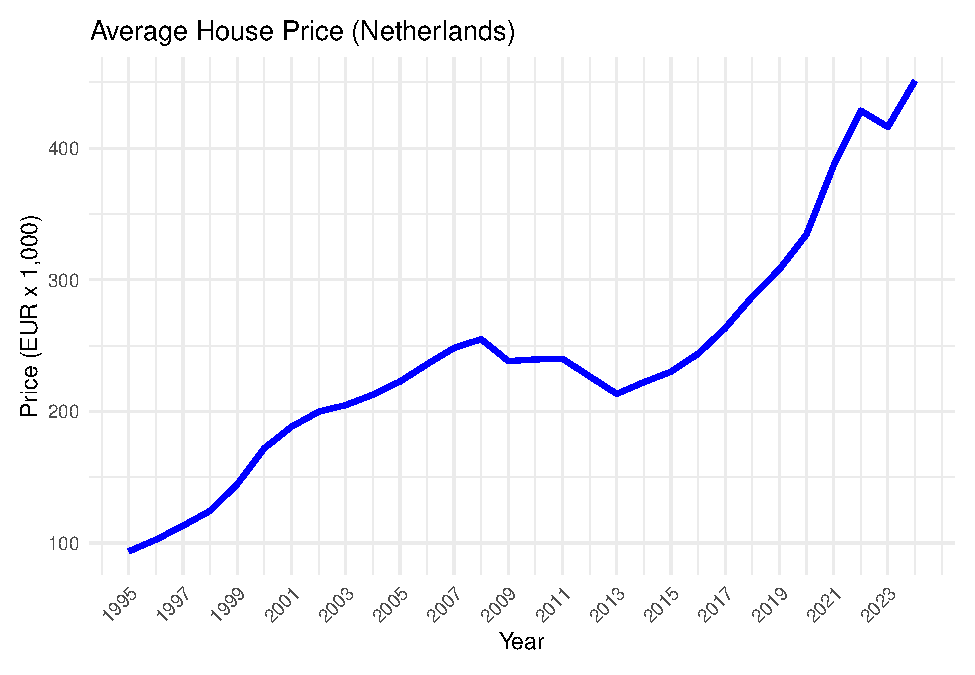
\includegraphics[width=0.52\linewidth,height=0.3\textheight]{rMarkdownProgrammingForEconomistsTutorial1Group6_files/figure-latex/visualise temporal variation-1}
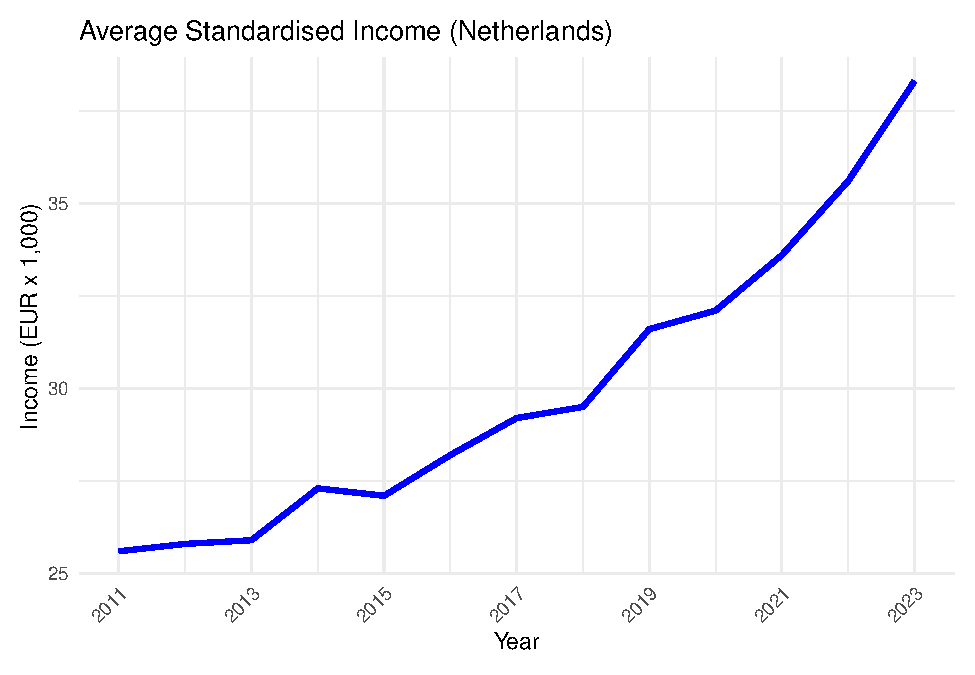
\includegraphics[width=0.52\linewidth,height=0.3\textheight]{rMarkdownProgrammingForEconomistsTutorial1Group6_files/figure-latex/visualise temporal variation-2}

The affordability of housing in the Netherlands has undergone
significant changes over time, as illustrated by the five temporal
visualisations. Figure 1 presents the development of average house
prices from 1995 to 2023, showing a steady upward trend, with
particularly sharp increases after 2015. Figure 2 complements this by
depicting the evolution of average standardised disposable income since
2011, which shows only moderate growth in comparison.

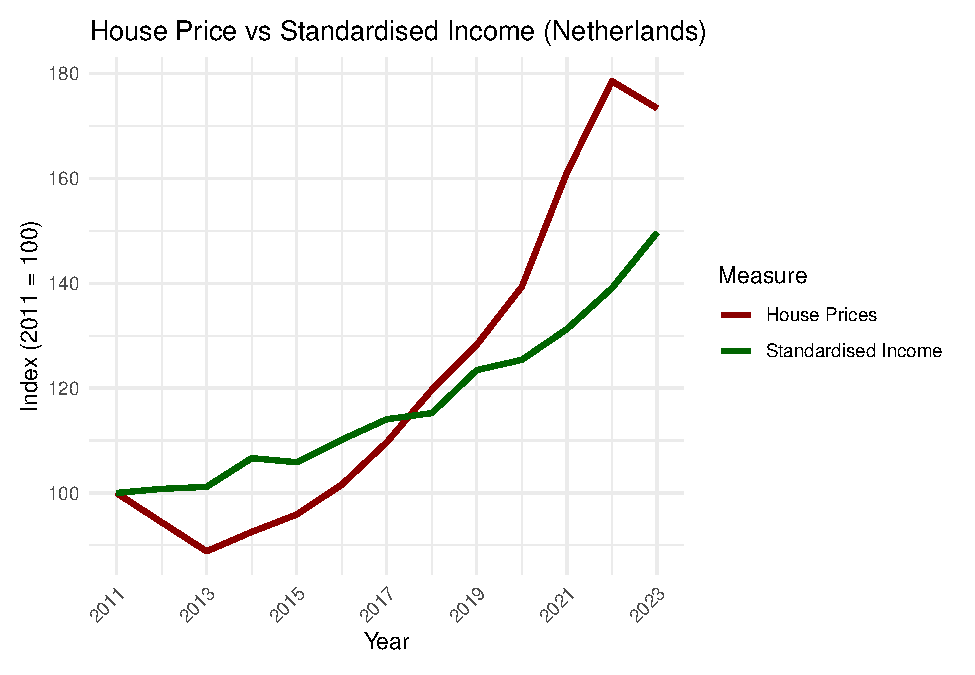
\includegraphics[width=0.52\linewidth,height=0.3\textheight]{rMarkdownProgrammingForEconomistsTutorial1Group6_files/figure-latex/visualise temporal variation two-1}
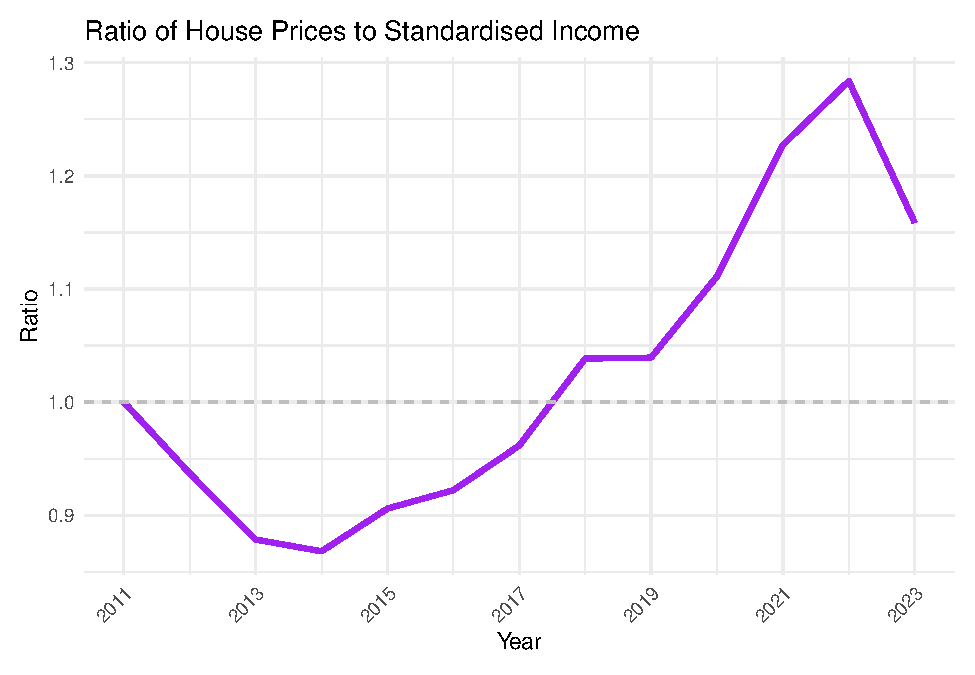
\includegraphics[width=0.52\linewidth,height=0.3\textheight]{rMarkdownProgrammingForEconomistsTutorial1Group6_files/figure-latex/visualise temporal variation two-2}

To better understand relative changes, Figure 3 presents both house
prices and income as indexed values (2011 = 100). This comparison
highlights that house prices have increased at a substantially faster
rate than incomes, especially after 2013, suggesting a growing mismatch
between the two variables. Finally, Figure 4 visualises the ratio of
house prices to standardised income over time. The upward trajectory of
this ratio indicates a declining affordability of housing, as house
prices increasingly outpace income levels. The dashed reference line at
a ratio of 1 serves as a benchmark: values above this threshold imply
deteriorating affordability.

\begin{center}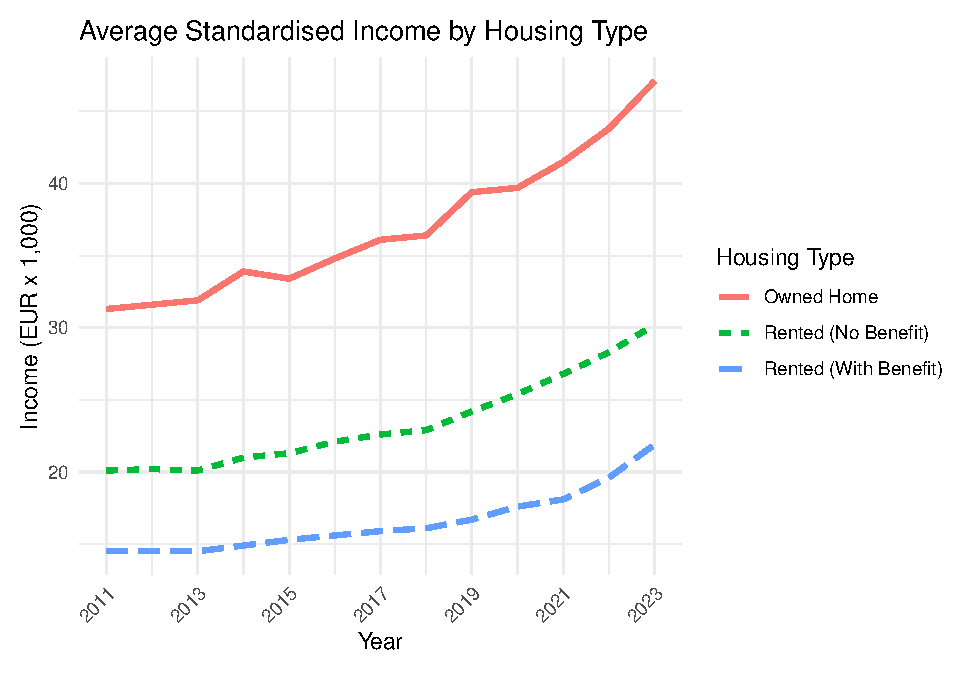
\includegraphics[width=0.52\linewidth,height=0.3\textheight]{rMarkdownProgrammingForEconomistsTutorial1Group6_files/figure-latex/visualise temporal variation three-1} \end{center}

The fifth visualisation presents average standardised income by housing
tenure over the period 2011--2023. While younger individuals typically
start their careers with lower incomes, this plot reveals that although
the relative income gap between housing types has remained stable, the
absolute difference in income levels between homeowners and renters has
grown substantially over the past twelve years. This growing absolute
gap exacerbates affordability challenges for lower-income renters, many
of whom are young adults or households yet to enter the property market.

These visualisations align closely with the research topic on housing
affordability, providing clear evidence of a growing temporal gap
between income and house prices. Time is consistently displayed on the
x-axis, ensuring the temporal dimension is appropriately represented.

\subsection{3.4 Visualise spatial
variation}\label{visualise-spatial-variation}

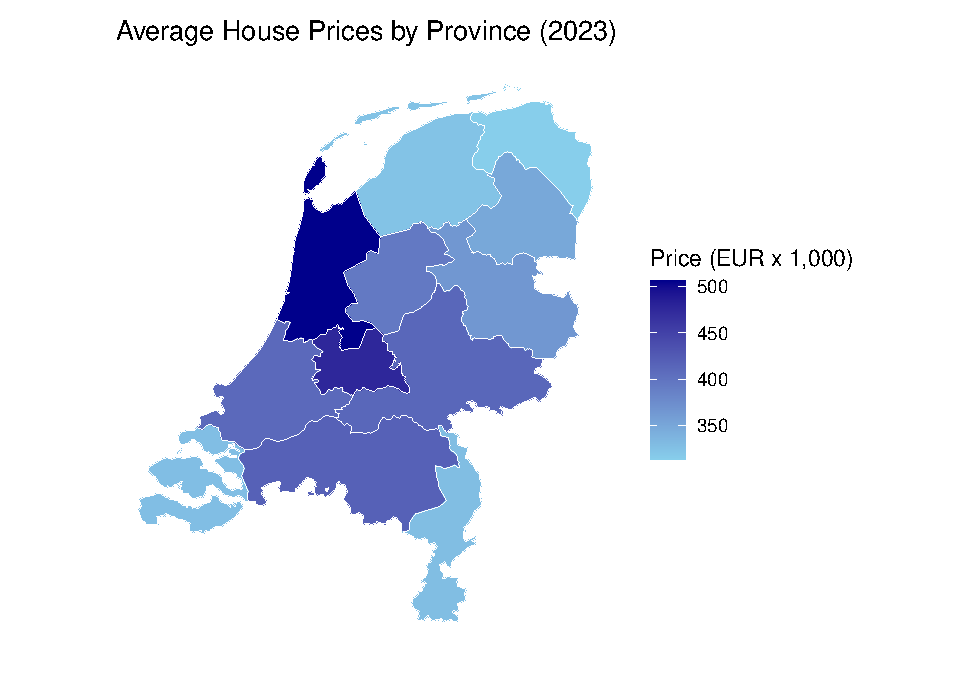
\includegraphics[width=0.52\linewidth,height=0.3\textheight]{rMarkdownProgrammingForEconomistsTutorial1Group6_files/figure-latex/visualise spatial variation-1}
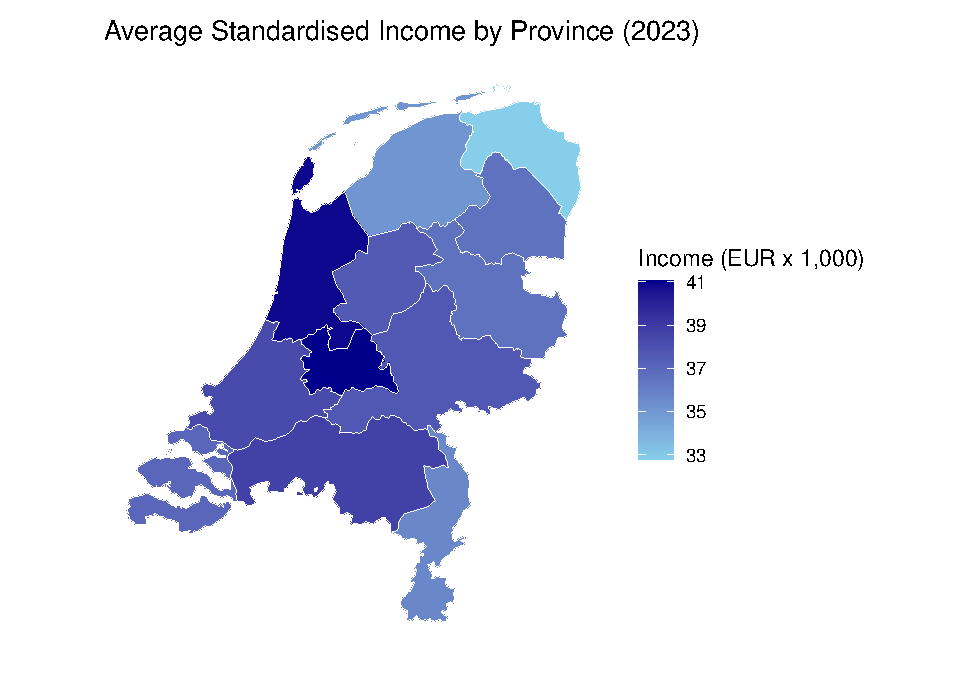
\includegraphics[width=0.52\linewidth,height=0.3\textheight]{rMarkdownProgrammingForEconomistsTutorial1Group6_files/figure-latex/visualise spatial variation-2}

The spatial visualisations above demonstrate how the problem of housing
affordability varies across the provinces of the Netherlands in 2023.
Figure 1 shows average house prices by province, indicating that housing
is most expensive in the Randstad area---particularly in North Holland,
South Holland, and Utrecht---while prices are relatively lower in
peripheral provinces such as Groningen, Friesland, and Drenthe.

Figure 2 displays the average standardised disposable income across the
same provinces. Although higher income levels are also concentrated in
the western part of the country, the regional relative variation in
income is notably smaller than the relative variation in house prices.
This imbalance implies that housing affordability issues are most severe
in provinces where house prices significantly exceed income levels.

This visualisation aligns with the topic of housing affordability by
highlighting the spatial mismatch between house prices and incomes,
helping to identify which regions face the greatest challenges. Mapping
these indicators at the provincial level provides a clear geographic
perspective on affordability, supporting evidence-based analysis of
regional disparities.

\subsection{3.5 Visualise sub-population
variation}\label{visualise-sub-population-variation}

\begin{center}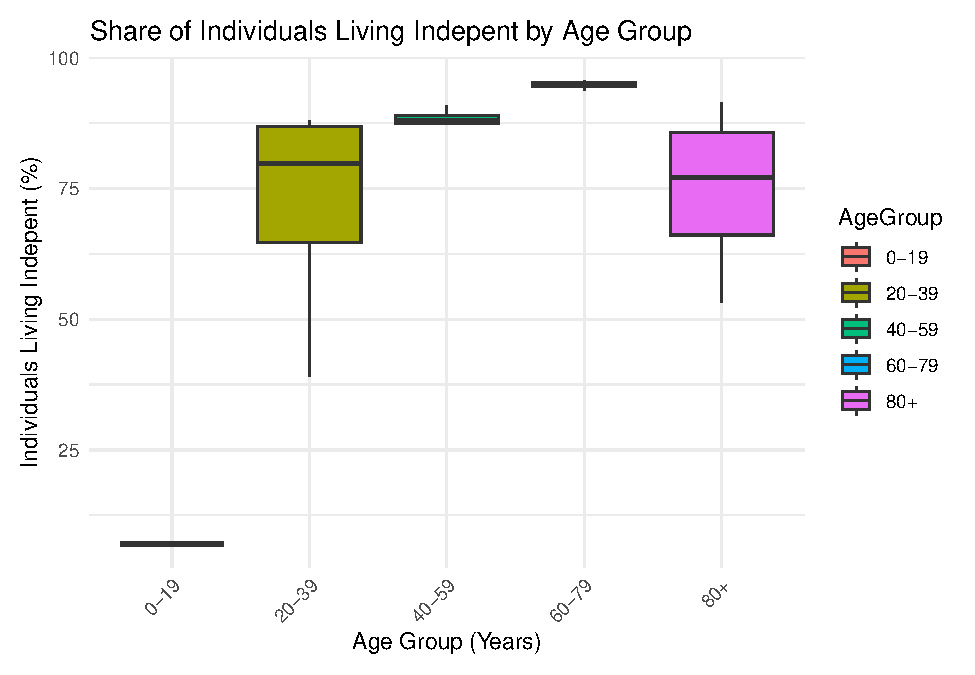
\includegraphics[width=0.52\linewidth,height=0.3\textheight]{rMarkdownProgrammingForEconomistsTutorial1Group6_files/figure-latex/visualise subpopulations-1} \end{center}

The boxplot visualises the distribution of the percentage of individuals
living independently across five broad age groups. The 40--59 and 60--79
age groups show the highest and most consistent rates of independent
living, with medians close to or above 90\%. In contrast, the 0--19 age
group has an extremely low share, reflecting that nearly all individuals
in this group live dependently. The 20--39 and 80+ groups exhibit wider
variability: for 20--39-year-olds, this suggests a transition period
where many begin living independently at differing rates; for the 80+
group, the spread may reflect differences in health, support needs, or
institutional living arrangements. This visualisation aligns closely
with the topic of housing affordability by demonstrating that the
problem manifests unevenly across sub-populations defined by age and
housing tenure. The grouped plot and the selected variables effectively
highlight how demographic and economic factors contribute to
differential affordability pressures within the Dutch housing market.

\subsection{3.6 Event analysis}\label{event-analysis}

\begin{center}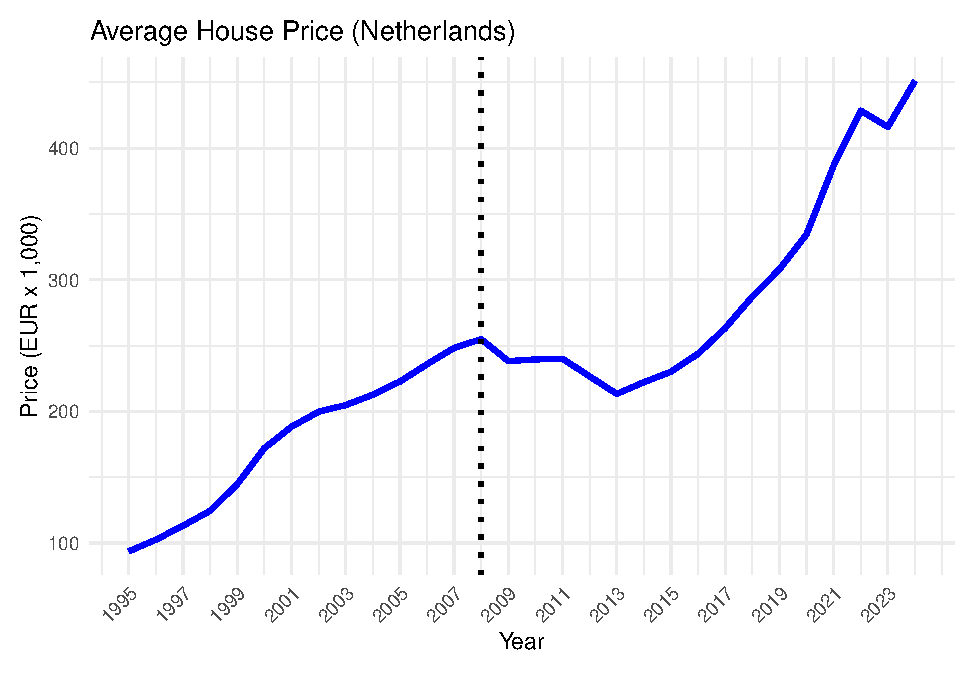
\includegraphics[width=0.52\linewidth,height=0.3\textheight]{rMarkdownProgrammingForEconomistsTutorial1Group6_files/figure-latex/event-analysis-1} \end{center}

The event analysis visualisation depicts average house prices in the
Netherlands over time, with a specific focus on the year 2008, marked by
a vertical dotted line. This year corresponds to the global financial
crisis, a significant event that had a marked impact on housing markets
worldwide.

Before 2008, house prices exhibited a steady upward trend. However, the
visualisation shows a clear disruption around this event: house prices
plateaued and even declined briefly following 2008, reflecting the
crisis's immediate effect on the housing market. After this period,
prices resumed their upward trajectory, but with increased volatility
and sharper increases in subsequent years.

This visualisation is directly relevant to the topic of housing
affordability, as it highlights how a major economic event can
temporarily alter housing price dynamics. The post-crisis acceleration
in prices, despite income growth remaining comparatively modest,
suggests that affordability pressures intensified after 2008.
Understanding such event-driven changes is critical for analysing the
temporal fluctuations and risks inherent in the housing market.

\section{Part 4 - Discussion}\label{part-4---discussion}

The results presented in the previous sections offer a comprehensive and
multidimensional view of housing affordability in the Netherlands.
Through the combination of temporal, spatial, and demographic analyses,
several critical patterns emerge that warrant closer reflection.

First, the temporal visualisations clearly show a persistent and
widening gap between house prices and standardised income over the last
decade. While house prices have increased substantially since 2013,
average standardised income has only grown modestly. This decoupling of
income from housing costs has resulted in a steadily rising
affordability ratio, particularly after 2015, indicating that housing is
becoming less accessible for many Dutch residents. These findings
support the concerns highlighted in Part 1, where growing generational
inequality and the increasing economic marginalisation of middle-income
households were described. The index-based approach
\texttt{(2011\ =\ 100)} proves useful in quantifying the speed and
direction of these divergent trends over time.

The spatial dimension further emphasises the imbalance. House prices in
the Randstad provinces (North Holland, South Holland, Utrecht) are
significantly higher than in peripheral regions, yet the variation in
income across provinces is much narrower. This implies that
affordability problems are particularly acute in urban and economically
dynamic regions, where housing demand outpaces supply. These spatial
discrepancies are consistent with the national housing shortage
identified by CBS and raise concerns about regional inequality and
spatial segregation.

Demographically, the sub-population analysis reveals that affordability
constraints affect age groups differently. Younger age cohorts (20--39)
show considerable variation in independent living, suggesting that
structural barriers---such as unaffordable housing---may be delaying
household formation and economic independence. This demographic
stagnation, especially among young adults, aligns with existing
literature on declining homeownership rates and delayed life course
transitions. The high consistency of independent living in middle-aged
groups underscores that affordability challenges are disproportionately
burdening newer market entrants.

The event analysis adds further nuance by highlighting the impact of the
2008 global financial crisis. While house prices temporarily stabilised
or declined during this period, the recovery phase was marked by
accelerated price increases, without a commensurate rise in income. This
pattern suggests a long-term structural shift rather than a cyclical
fluctuation. Moreover, the visual break in the trend underscores the
vulnerability of the housing market to external shocks, reinforcing the
need for resilience-oriented housing policy.

While the findings are robust, several limitations should be
acknowledged. The inconsistent temporal coverage across datasets reduces
the potential for long-term integrated analysis, particularly prior to
2011. Furthermore, administrative data, while rich and reliable, may
fail to capture informal housing arrangements or underrepresented
subpopulations such as undocumented migrants or those in non-traditional
living setups. Additionally, the income measures used do not account for
wealth accumulation (e.g., equity from homeownership), which may further
differentiate affordability across households.

Nevertheless, the constructed indices and affordability ratio offer
powerful tools for quantifying and comparing affordability over time,
across regions, and between demographic groups. They provide a rigorous
empirical foundation for policy evaluation and highlight where
interventions may be most needed---namely in urbanised provinces, among
young adults, and in the private rental sector where income constraints
are most acute.

Future research could incorporate micro-level data on housing
expenditures, debt burdens, or wealth to enrich the analysis. Moreover,
evaluating the role of government policies (e.g., housing subsidies,
rent control, zoning regulations) could offer valuable insights into
potential levers for improving affordability.

In summary, the Dutch housing market has become increasingly
unaffordable over the past decade, particularly for younger and
lower-income populations. The widening gap between housing costs and
incomes, compounded by spatial and demographic disparities, presents a
pressing social and economic challenge. Addressing this issue will
require a combination of data-informed policy reforms and targeted
investments to restore affordability and equity in the housing system.

\section{Part 5 - Reproducibility}\label{part-5---reproducibility}

\subsection{5.1 Github repository link}\label{github-repository-link}

Github link:
\url{https://github.com/Daan-Blok/ProgrammingForEconomists.git}

\subsection{5.2 Reference list}\label{reference-list}

Wat zijn gevolgen van de onzekere woningmarkt voor jongeren? \textbar{}
Nederlands Jeugdinstituut. (n.d.-b).
\url{https://www.nji.nl/op-jezelf-wonen/wat-zijn-gevolgen-van-de-onzekere-woningmarkt-voor-jongeren}

Wiesel, I., Ralston, L., \& Stone, W. (2021). Understanding
after-housing disposable income effects on rising inequality. Housing
Studies, 38(2), 290--306.
\url{https://doi.org/10.1080/02673037.2021.1882661}

Schilder, F., Scherpenisse, R., PBL Netherlands, \& Tiwos. (n.d.).
Affordable housing in the Netherlands.
\url{https://www.pbl.nl/sites/default/files/downloads/PBL2018_Policy-and-practice-affordable-housing-in-the-Netherlands_3336_0.pdf}

Pouwels-Urlings, N. (2021, April 20). \emph{Herziening van de
Vermogensstatistiek 2006}. Centraal Bureau Voor De Statistiek.
\url{https://www.cbs.nl/nl-nl/longread/discussion-papers/2021/herziening-van-de-vermogensstatistiek-2006}
(86004NED)

\emph{CBS dataportaal}. (n.d.-c).
\url{https://opendata.cbs.nl/statline/portal.html?_la=nl&_catalog=CBS&tableId=86004NED&_theme=310\#}

Centraal Bureau voor de Statistiek. (2008). Prijsindex bestaande
koopwoningen methodebeschrijving. In \emph{Prijsindex Bestaande
Koopwoningen Methodebeschrijving}.
\url{https://www.cbs.nl/-/media/_pdf/2018/08/methodebeschrijving-prijsindex-bestaande-koopwoningen.pdf}
(83625NED)

\emph{CBS dataportaal}. (n.d.).
\url{https://opendata.cbs.nl/statline/portal.html?_la=nl&_catalog=CBS&tableId=83625NED&_theme=398\#}

Bakker, B. F., Van Rooijen, J., \& Van Toor, L. (2014). The System of
social statistical datasets of Statistics Netherlands: An integral
approach to the production of register-based social statistics.
\emph{Statistical Journal of the IAOS}, \emph{30}(4), 411--424.
\url{https://doi.org/10.3233/sji-140803} (71488ned)

\emph{CBS dataportaal}. (n.d.-b).
\url{https://opendata.cbs.nl/statline/portal.html?_la=nl&_catalog=CBS&tableId=71488ned&_theme=281\#}

\end{document}
